\documentclass[11pt]{beamer}

%% Sprache und Zeichensatz:
\usepackage[applemac]{inputenc}
%\usepackage[ngerman]{babel}
\usepackage[T1]{fontenc}
\usepackage[ngerman,english]{babel}
\usepackage{lmodern}

\usepackage{amsmath}
\usepackage{amssymb}
\usepackage{amstext}
%\usepackage{amsthm}

\usepackage{setspace}

\usetheme{boxes}
\usepackage{dsfont}

\usecolortheme{rose}
\useinnertheme[shadow]{rounded}

%---------------------------------------------------------------------------------------------
%
%%Pakete Mathematik
%\usepackage{amsmath, amssymb, amstext, amsfonts, mathrsfs}
%\usepackage[squaren]{SIunits}

%---------------------------------------------------------------------------------------------
%% F�r eine Titelseite:

%%%%%%

\usepackage[matrix,arrow]{xy}
\usepackage{stmaryrd}

\DeclareMathOperator*{\esssup}{ess.sup}
\DeclareMathOperator*{\defgl}{:=}
\DeclareMathOperator*{\defgr}{=:}
\DeclareMathOperator*{\argmax}{argmax}

\newcommand{\3}{ ^{3\times3} }
\newcommand{\R}{\mathbb{R}}
\newcommand{\N}{\mathbb{N}}
\newcommand{\M}{\mathbb{M}}
\newcommand{\Sym}{\mathbb{S}^3}
\newcommand{\Mpos}{\M_+^3}
\newcommand{\Orth}{\mathbb{O}^3}
\newcommand{\norm}[1]{\left\lVert#1\right\rVert}
\newcommand{\abs}[1]{\left |#1\right |}
\newcommand{\ub}{\bar{u}}
\newcommand{\yb}{\bar{y}}
\newcommand{\scprod}[2]{\langle#1 , #2 \rangle}
\newcommand{\E}{\mathcal{E}}
\newcommand{\F}{\mathcal{F}}
\newcommand{\G}{\mathcal{G}}


% TIKZ DIAGRAMS

\usepackage{tikz}
\usetikzlibrary{arrows}
\usetikzlibrary{positioning}

\tikzset{
    block/.style={
           rectangle,
           rounded corners,
           draw=black, very thick,
           minimum height=2em,
           inner sep=2pt,
           text centered,
           },
     block2/.style={
           %rectangle,
           %rounded corners,
           fill=black!20,
           %draw=black, very thick,
           minimum height=2em,
           inner sep=2pt,
           text centered,
           },
     frameless/.style={
           %rectangle,
           %rounded corners,
           %draw=black, very thick,
           minimum height=2em,
           inner sep=2pt,
           text centered,
           },
}

\usepackage{tikz-cd}
\tikzset{
  shift left/.style ={commutative diagrams/shift left={#1}},
  shift right/.style={commutative diagrams/shift right={#1}}
}



%%%%%%

\title{High Performance Computing Project\\ Parallelization of the Probabilistic Roadmap Method with GPU Acceleration} 
\author{Manuel Demmeler}
\institute{Technische Universit�t M�nchen}
\date{}


\AtBeginSection[]{ 
	\frame {
		%\frametitle{Gliederung}
		\tableofcontents[current, currentsubsection]
	} 
}

\begin{document}

\frame{\titlepage}


\begin{frame}
	\frametitle{Gliederung}
	\tableofcontents
\end{frame}

%%%%%%%%%%%%%%%%%%%%%%%
\section{Motivation}
\begin{frame}
\frametitle{Motivation}
	\begin{center}
		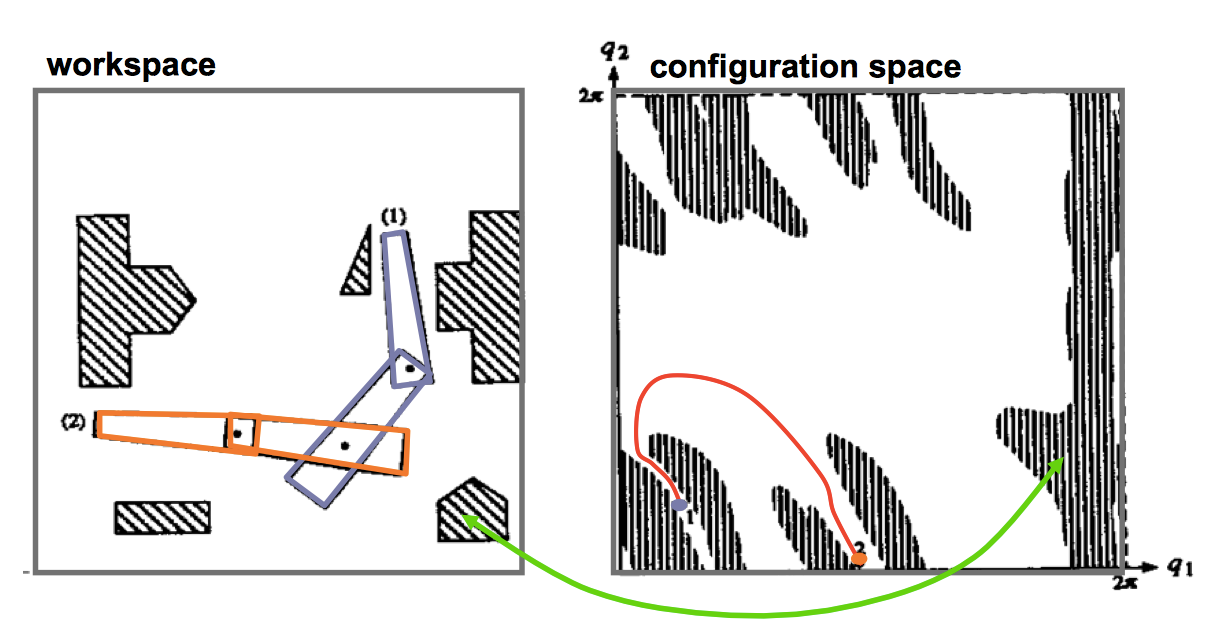
\includegraphics[height=4cm]{configspacetrafo.png}
	\end{center}
	\begin{itemize}
		\item Problem: find a feasible trajectory of a robot through a setting of obstacles
		\item often necessary to pass feasible initial tajectories to optimization algorithms
	\end{itemize}
\end{frame}

\newtheorem*{defi}{Definition}

\begin{frame}
\frametitle{Problem Statement}
	\begin{itemize}
		\item Obstacles can not be assumed to have a closed form
		\item Therefore they are defined by an indicator function
		\begin{equation*}
			I: \Omega \subset \R^d \rightarrow \{ 0,1 \}
		\end{equation*}
		\item collision for $q \in \Omega$, $I(q) = 1$ 
	\end{itemize}

\end{frame}

\begin{frame}
\frametitle{PRM Algorithm}
	PRM: Grow graphs from given start and endpoints $q_s, q_e \in \Omega$ until a connection is found, by repeating
	\begin{itemize}
		\item sample new node $v$ randomly in environment of old nodes
		\item check for all possible neighbors $w$, if the linear connection is feasible, in this case add edge $\{v,w\}$ to the graph
		\item break, if the two graphs have been connected.
	\end{itemize}
	\begin{defi}
	For two points \(v\) and \(w\) we define the connection with stepsize \(h>0\) as
		\begin{equation*}
			[v,w]_h \defgl \{ q = \lambda v+(1-\lambda) w\ |\ \lambda \in [0,1], \norm{q-v} \in \N_0 h \}.
		\end{equation*}
		We say, \(q_1\) and \(q_2\) are connected with stepsize \(h>0\), if
		\(I(q)=0\) for all \(q \in [q_1, q_2]_h\).
	\end{defi}
\end{frame}

%%%%%%%%%%%%%%%%%%%%%%%
\section{Robotics Application}
\begin{frame}
\frametitle{Robotics Application}
	\begin{center}
		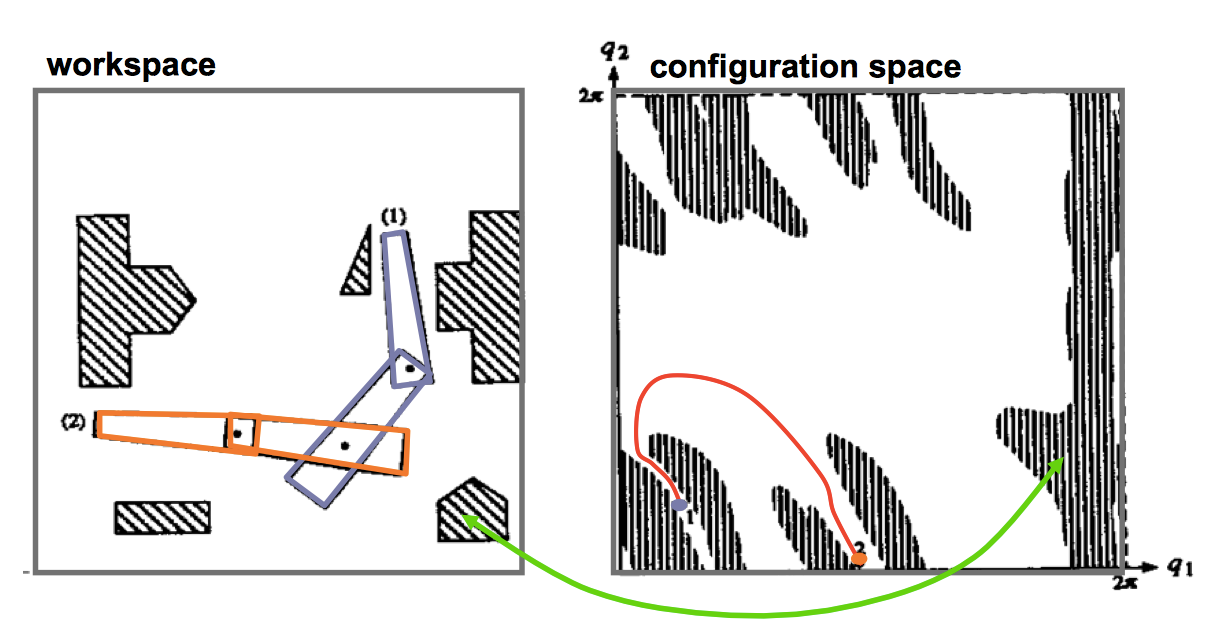
\includegraphics[height=3cm]{configspacetrafo.png}
	\end{center}
	\begin{itemize}
		\item For each linear connection, every intermediate configuration has to be checked for collisions
		\item $\Rightarrow$ Many independent and similar kinematics and collision calculations
		\item $\Rightarrow$ Well suited for usage of GPU
	\end{itemize}
\end{frame}


\begin{frame}
\frametitle{Project Overview}
\begin{center} 
\resizebox{\textwidth}{!}{%
\begin{tikzpicture}[auto]%node distance=0.5cm and 1.8cm]
	\node[block] (prm) {
		\begin{tabular}{c}
		\textbf{PRMSolver}\\
		generate nodes\\
		store graph
		\end{tabular}
	};
	\node [block, right=of prm] (config) {
		\begin{tabular}{c}
		\textbf{Configpace}\\
		indicator fct. \\
		interface
		\end{tabular}
	};
	\node [block, right=of config] (robo) {
		\begin{tabular}{c}
		\textbf{RobotConfigspace}\\
		robot kinematics\\
		collision detection
		\end{tabular}
	};
	\node [block, right=of robo] (gpu) {\textbf{GPU}};
	
	\path[-stealth,thick, shift left=1.0ex]	(prm) edge (config) ;
	\path[-stealth,thick, shift left=1.0ex]	(config) edge  (prm) ;
	\path[-stealth,thick, shift left=1.0ex]	(config) edge (robo);
	\path[-stealth,thick, shift left=1.0ex]	(robo) edge  (config);
	\path[-,thick]					(robo) edge (gpu);
\end{tikzpicture}
}
\end{center}
	\begin{itemize}
	\item PRM algorithm and Configuration space independent from each other
	\item Only connected through indicator function represented by Configspace interface
	\end{itemize}
\end{frame}


\begin{frame}
\frametitle{Second Level of Parallelization}
	Version 1:
	\begin{itemize}
	\item Use multiple GPUs parallely
	\item Sample and connect new nodes on each processor
	\item Exchange nodes and edges
	\end{itemize}
	
\begin{center}
\resizebox{\textwidth}{!}{%
\begin{tikzpicture}[auto, node distance=0.5cm and 1.8cm]
	\node[block, minimum width=3cm] (prm) {
		\begin{tabular}{c}
		\textbf{PRMSolver 1}
		\end{tabular}
	};
	
	\node[frameless, below=of prm, minimum width=3cm] (space) {$\vdots$};
	
	\node[block, below=of space, minimum width=3cm] (prm2) {
		\begin{tabular}{c}
		\textbf{PRMSolver n}
		\end{tabular}
	};
	
	\node [block, right=of prm] (config) {
		\begin{tabular}{c}
		\textbf{Configpace 1}
		\end{tabular}
	};
	\node[frameless, below=of config] (space2) {$\vdots$};
	\node [block, below=of space2] (config2) {
		\begin{tabular}{c}
		\textbf{Configpace n}
		\end{tabular}
	};
	
	
	
	\node [block, right=of config] (gpu) {\textbf{GPU 1}};
	\node [block, right=of config2] (gpu2) {\textbf{GPU n}};
	
	
	\path[-latex',thick, shift left=1.0ex]	(prm) edge (config) 
								(config) edge (prm);
	\path[-,thick]					(config) edge (gpu);
	
	\path[-latex',thick, shift left=1.0ex]	(prm2) edge (config2) 
								(config2) edge (prm2) ;
	\path[-,thick]					(config2) edge (gpu2);
	
	
	\path[-latex',thick, shift left=1.0ex]	(prm) edge (space)
								(space) edge (prm)
								(prm2) edge (space)
								(space) edge (prm2) ;
	

\end{tikzpicture}
}
\end{center}

\end{frame}

\begin{frame}
\frametitle{Second Level of Parallelization}
	Version 2:
	\begin{itemize}
		\item Grow whole graphs on every processor
		\item Exchange only edges
	\end{itemize}
\begin{center}
\resizebox{\textwidth}{!}{%
\begin{tikzpicture}[auto, node distance=0.5cm and 1.8cm]
	\node[block, minimum width=3cm] (prm) {
		\begin{tabular}{c}
		\textbf{PRMSolver 1}
		\end{tabular}
	};
	
	\node[frameless, below=of prm, minimum width=3cm] (space) {$\vdots$};
	
	\node[block, below=of space, minimum width=3cm] (prm2) {
		\begin{tabular}{c}
		\textbf{PRMSolver n}
		\end{tabular}
	};
	
	\node [block, right=of prm] (config) {
		\begin{tabular}{c}
		\textbf{Configpace 1}
		\end{tabular}
	};
	\node[frameless, below=of config] (space2) {$\vdots$};
	\node [block, below=of space2] (config2) {
		\begin{tabular}{c}
		\textbf{Configpace n}
		\end{tabular}
	};
	
	
	
	\node [block, right=of config] (gpu) {\textbf{GPU 1}};
	\node [block, right=of config2] (gpu2) {\textbf{GPU n}};
	
	
	\path[-latex',thick, shift left=1.5ex]	(prm) edge (config) ;
	\path[-,thick]					(config) edge (gpu);
	
	\path[-latex',thick, shift right=1.5ex]	(prm2) edge (config2) ;
	\path[-,thick]					(config2) edge (gpu2);
	
	
	\path[-latex',thick]				(config.west) edge  (prm.east) 
								(config.west) edge (space.east)
								(config.west) edge (prm2.east)
								(config2.west) edge  (prm.east) 
								(config2.west) edge (space.east)
								(config2.west) edge (prm2.east);

\end{tikzpicture}
}
\end{center}
\end{frame}

\begin{frame}
\frametitle{Implementation and Testing}
	\begin{itemize}
	\item GPU imlementation with CUDA
	\item CPU Parallelization with MPI
	\item Tested with a 4 axis robot scenario created with CAD/Matlab
	\end{itemize}
	\begin{center}
	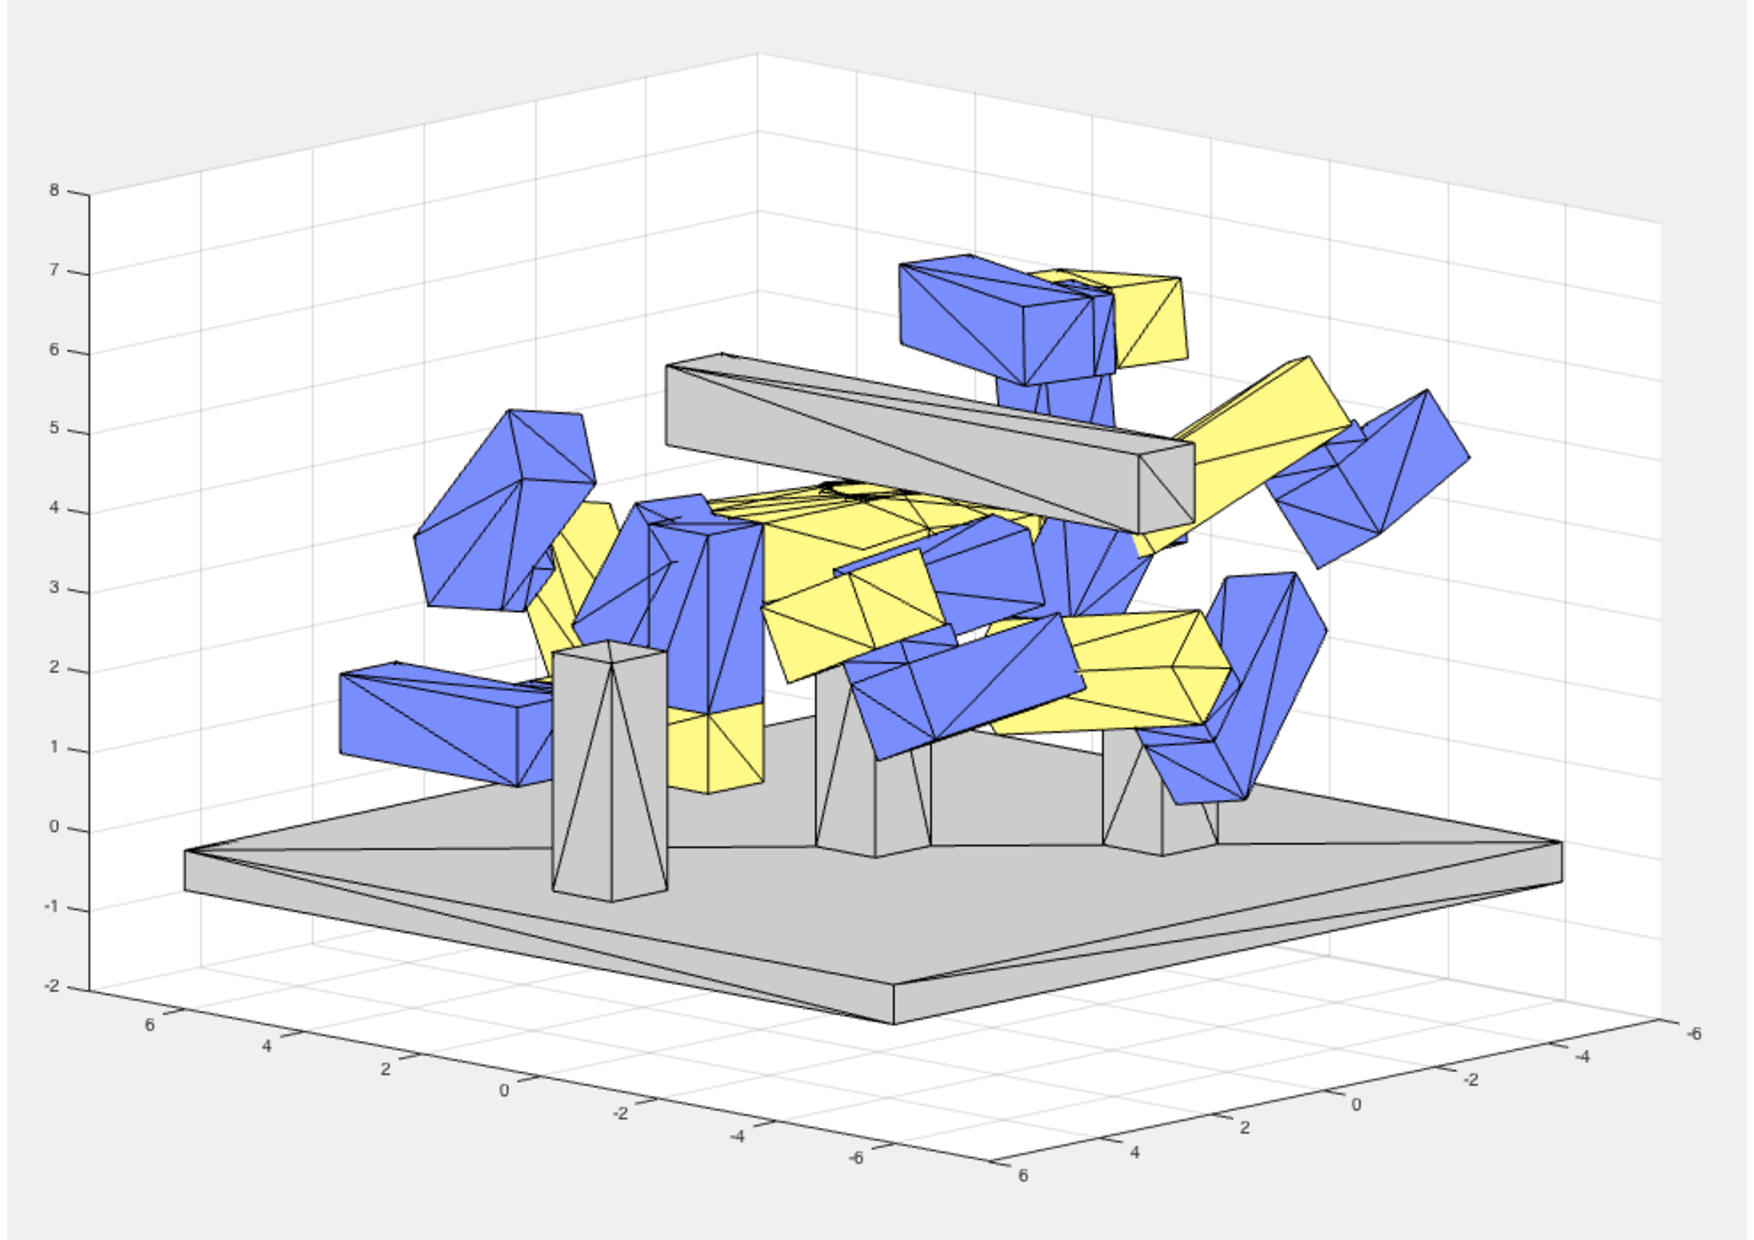
\includegraphics[height=4cm]{robotsolution.pdf}
	\end{center}
\end{frame}


\begin{frame}
\frametitle{Literatur}
\bibliographystyle{alpha}
\begin{thebibliography}{999}
	\bibitem{prmlec} D. Burschka, Lecture Robot Motion Planning, source: http://robvis01.informatik.tu-muenchen.de/courses/wegtraj/index.html
	\bibitem{prm1} H. Choset, K. Lynch, S. Hutchinson, G. Kantor, W. Burgard, L. Kavraki and S. Thrun, Principles of Robot Motion: Theory, Algorithms, and Implementation, MIT Press, 2005
	\bibitem{prm2} S. M. LaValle, Planning Algorithms, Cambridge University Press, 2006
	\bibitem{robodyn} T. Buschmann, Skript zur Vorlesung: Roboterdynamik SS14, Lehrstuhl f�r Angewandte Mechanik, TU M�nchen, 2014
	\bibitem{chung} K. Chung, Wenping Wang, Quick Collision Detection of Polytopes in Virtual Environments, Proceedings of the ACM Symposium on Virtual Reality Software and Technology (VRST 96), Mark Green (ed.), 1996
	\bibitem{ericson} C. Ericson, Real-Time Collision Detection, Elsevier, 2005
\end{thebibliography}
\end{frame}


\end{document}
















